\documentclass{standalone}
\usepackage{tikz}
\usetikzlibrary{calc,matrix}

\definecolor{bluecol}{RGB}{124,156,205}
\definecolor{greencol}{RGB}{149,178,1}
\definecolor{redcol}{RGB}{216,157,125}
\definecolor{yellowcol}{RGB}{219,193,0}

\tikzset{
  table/.style={
    matrix of nodes,
    row sep=-\pgflinewidth,
    column sep=-\pgflinewidth,
    nodes={rectangle,text width=1.8cm,align=center},
    text depth=1.25ex,
    text height=2.5ex,
    nodes in empty cells
  },
  border/.style={white,ultra thick},
  label/.style={font={\footnotesize\sffamily\bfseries\color{white}}},
  bcell/.style={fill=bluecol},
  ycell/.style={fill=yellowcol},
  gcell/.style={fill=greencol},
  rcell/.style={fill=redcol},
}

\renewcommand*{\familydefault}{\sfdefault}

\begin{document}

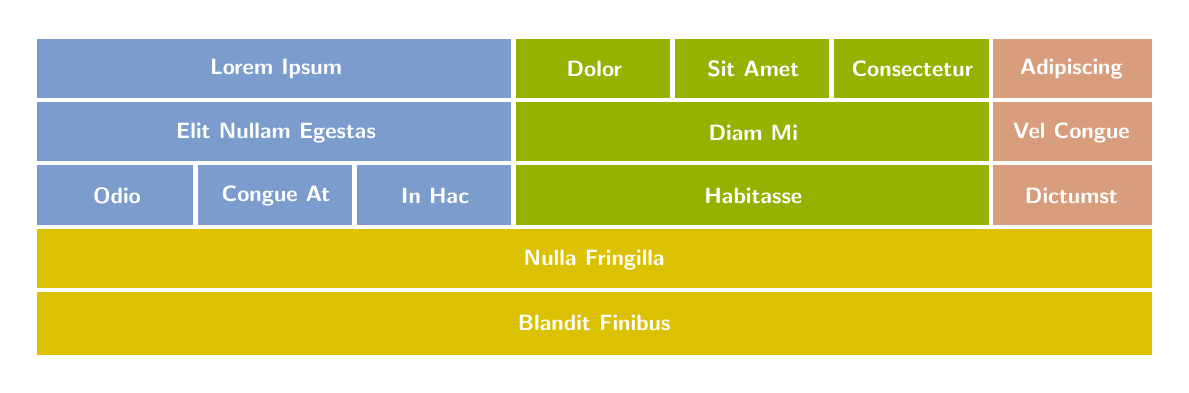
\begin{tikzpicture}
  \matrix (mat) [table] {
    |[bcell]| & |[bcell]| & |[bcell]| & |[gcell]|  & |[gcell]| & |[gcell]|  & |[rcell]|  \\
    |[bcell]| & |[bcell]| & |[bcell]| & |[gcell]|  & |[gcell]| & |[gcell]|  & |[rcell]|  \\
    |[bcell]| & |[bcell]| & |[bcell]| & |[gcell]|  & |[gcell]| & |[gcell]|  & |[rcell]|  \\
    |[ycell]| & |[ycell]| & |[ycell]| & |[ycell]|  & |[ycell]|  & |[ycell]| & |[ycell]|  \\
    |[ycell]| & |[ycell]| & |[ycell]| & |[ycell]|  & |[ycell]|  & |[ycell]| & |[ycell]|  \\
  };

  \foreach \row in {1,2,3,4,5}
    \draw[border] (mat-\row-1.north west) -- (mat-\row-7.north east);
  \foreach \col in {5,6,7}
    \draw[border] (mat-1-\col.north west) -- (mat-1-\col.south west);
  \foreach \col in {2,3}
    \draw[border] (mat-3-\col.north west) -- (mat-3-\col.south west);
  \foreach \col in {4,7}
    \draw[border] (mat-1-\col.north west) -- (mat-3-\col.south west);

  \node[label] at (mat-1-2) {Lorem Ipsum}; ,
  \node[label] at (mat-1-4) {Dolor};
  \node[label] at (mat-1-5) {Sit Amet};
  \node[label] at (mat-1-6) {Consectetur};
  \node[label] at (mat-1-7) {Adipiscing};

  \node[label] at (mat-2-2) {Elit Nullam Egestas};
  \node[label] at (mat-2-5) {Diam Mi};
  \node[label] at (mat-2-7) {Vel Congue};

  \node[label] at (mat-3-1) {Odio};
  \node[label] at (mat-3-2) {Congue At};
  \node[label] at (mat-3-3) {In Hac};
  \node[label] at (mat-3-5) {Habitasse};
  \node[label] at (mat-3-7) {Dictumst};

  \node[label] at (mat-4-4) {Nulla Fringilla};

  \node[label] at (mat-5-4) {Blandit Finibus};
\end{tikzpicture}

\end{document}
